\documentclass[11pt]{article}

\usepackage{amsmath,amssymb,graphicx,booktabs,geometry,hyperref}
\geometry{margin=1in}
\graphicspath{{../}{./}}
\hypersetup{colorlinks=true, linkcolor=blue, urlcolor=blue}

\title{Homogeneous versus Spatial Mechanisms in an Eco-Evolutionary Predator--Prey PDE}
\author{Mathbio research notes}
\date{\today}

\begin{document}
\maketitle

\begin{abstract}
We test whether basin-dependent outcomes in a spatial eco-evolutionary predator--prey PDE are generated by persistent spatial structure or inherited from the homogeneous reaction system. The analysis uses the established parameterization, reuses saved representative PDE fields, compares matched ODE and PDE mean trajectories, quantifies spatial variance, compares ODE and PDE basin labels on the existing \(q_0\)--\(w_0\) grid, and runs a small perturbation-sensitivity test. The final decision label is \texttt{reaction\_dominated\_homogeneous\_multistability}. The observed PDE basins are primarily homogeneous reaction-dominated in this tested parameterization.
\end{abstract}

\section{Introduction}

The project has established that the well-mixed eco-evolutionary ODE can support indirect evolutionary rescue, while the fixed-defense spatial model did not produce robust spatial rescue. The spatial eco-evolutionary PDE can produce persistent, extinct, and transient outcomes at the same stress from different initial conditions. The unresolved mechanism question is whether these basins are truly spatially mediated or whether they are homogeneous reaction-system basins embedded in a PDE whose fields remain nearly uniform.

This report addresses that question directly. It does not change the equations, numerical parameter values, or representative case definitions. It also does not run broad parameter scans. The goal is a scoped mechanism diagnosis for the tested parameterization.

\section{Model and competing hypotheses}

Let \(n\) be total prey density, \(w\) predator density, \(q\) prey defense frequency, and
\[
z=\kappa^{-1}-n-w
\]
be free space. The defense-dependent functions are
\[
r(q)=r_u(1-q)+r_vq,\quad
a(q)=a_u(1-q)+a_vq,\quad
b(q)=b_u(1-q)+b_vq.
\]
The matched homogeneous ODE is
\begin{align}
\frac{dn}{dt} &= n\left[r(q)z-\xi-a(q)w\right],\\
\frac{dw}{dt} &= w\left[b(q)nz-(m+s)-\mu w\right],\\
\frac{dq}{dt} &= \nu q(1-q)\left[(r_v-r_u)z-(a_v-a_u)w\right].
\end{align}
The spatial PDE uses the same reaction terms with zero-flux diffusion:
\begin{align}
\partial_t n &= D_n\nabla^2 n+n\left[r(q)z-\xi-a(q)w\right],\\
\partial_t w &= D_w\nabla^2 w+w\left[b(q)nz-(m+s)-\mu w\right],\\
\partial_t q &= D_q\nabla^2 q+\nu q(1-q)\left[(r_v-r_u)z-(a_v-a_u)w\right].
\end{align}

The null hypothesis is reaction-dominated homogeneous multistability: the fields remain nearly homogeneous, PDE spatial means match ODE trajectories from the same initial mean, and basin labels agree. The spatial alternative is spatially mediated bistability: fields maintain nontrivial pattern strength, mean dynamics diverge, basin labels disagree systematically, or perturbation amplitude and seed alter basin entry.

\section{Numerical methods}

All calculations used \(\mathrm{RoyEvoParams}(b_u=0.08,b_v=0.02)\). The initial mean for each matched ODE trajectory was
\[
n(0)=n_\mathrm{baseline},\quad
w(0)=w_\mathrm{baseline}\,w_0^\mathrm{scale},\quad
q(0)=q_0,
\]
where the baseline comes from the same unstressed burn-in method used by the preceding PDE experiments. Representative PDE mean time series and final field archives were reused from the saved Step 19 outputs. The perturbation test used only the three representative cases, amplitudes \(0\), \(10^{-5}\), and \(10^{-3}\), and seeds 20260702 and 20260703, for 18 total PDE runs at \(T=1600\).

\section{Results}

\subsection{Matched ODE-PDE representative trajectories}

The matched representative comparison found 3 classification agreements out of 3 representative cases. The mean predator RMSE was 0.006409, and the maximum final predator-density difference was 7.102e-07.

\begin{table}[htbp]
\centering
\caption{Matched ODE and PDE representative classifications.}
\begin{tabular}{lllrr}
\toprule
Case & ODE classification & PDE classification & RMSE \(w\) & final \(|\Delta w|\) \\
\midrule
persistent\_case & \texttt{persistent\_steady} & \texttt{persistent\_steady} & 0.001009 & 7.144e-10 \\
extinct\_case & \texttt{extinct\_steady} & \texttt{extinct\_steady} & 3.098e-06 & 3.066e-12 \\
transient\_case & \texttt{recovery\_transient} & \texttt{recovery\_transient} & 0.01821 & 7.102e-07 \\
\bottomrule
\end{tabular}
\end{table}

\begin{figure}[htbp]
\centering
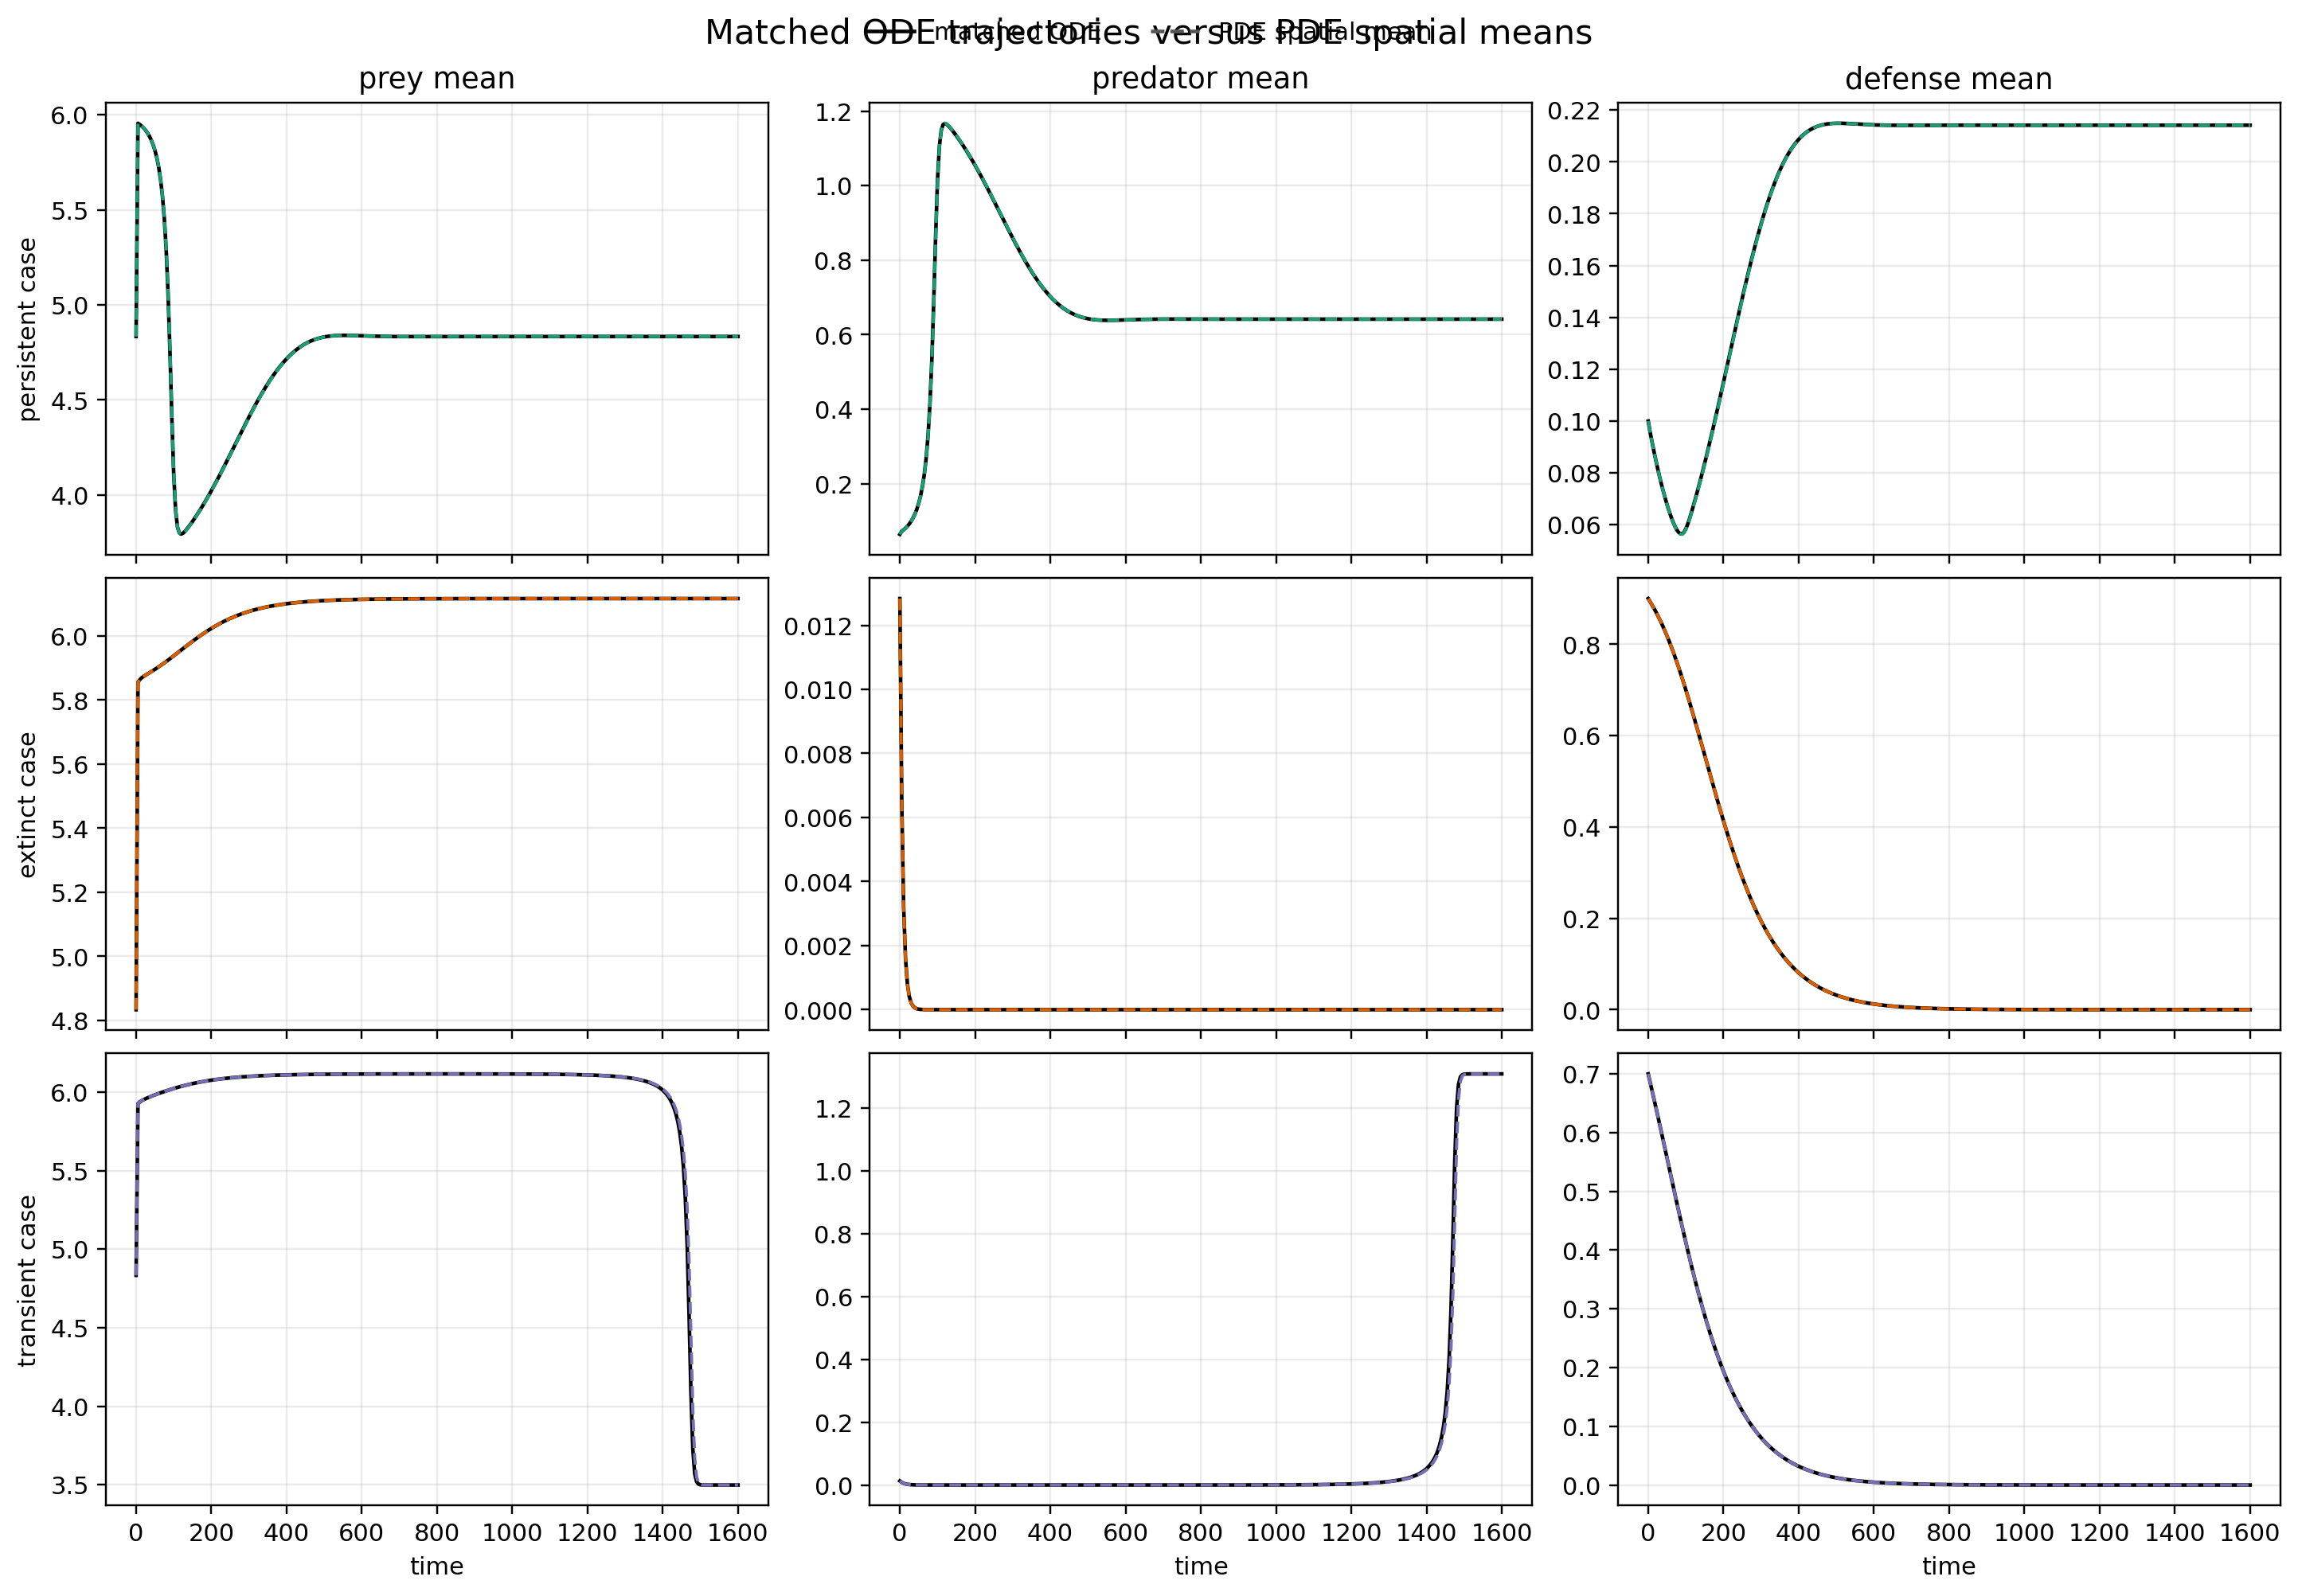
\includegraphics[width=0.98\linewidth]{figures/roy_evo_spatial/report/fig22_ode_pde_representative_comparison.png}
\caption{Matched ODE trajectories and PDE spatial means for representative persistent, extinct, and transient cases.}
\end{figure}

\subsection{Spatial variance and pattern strength}

Spatial coefficient of variation decayed to small values in the representative fields. The maximum final steady-case CV across \(n\), \(w\), and \(q\) was 3.101e-05.

\begin{figure}[htbp]
\centering
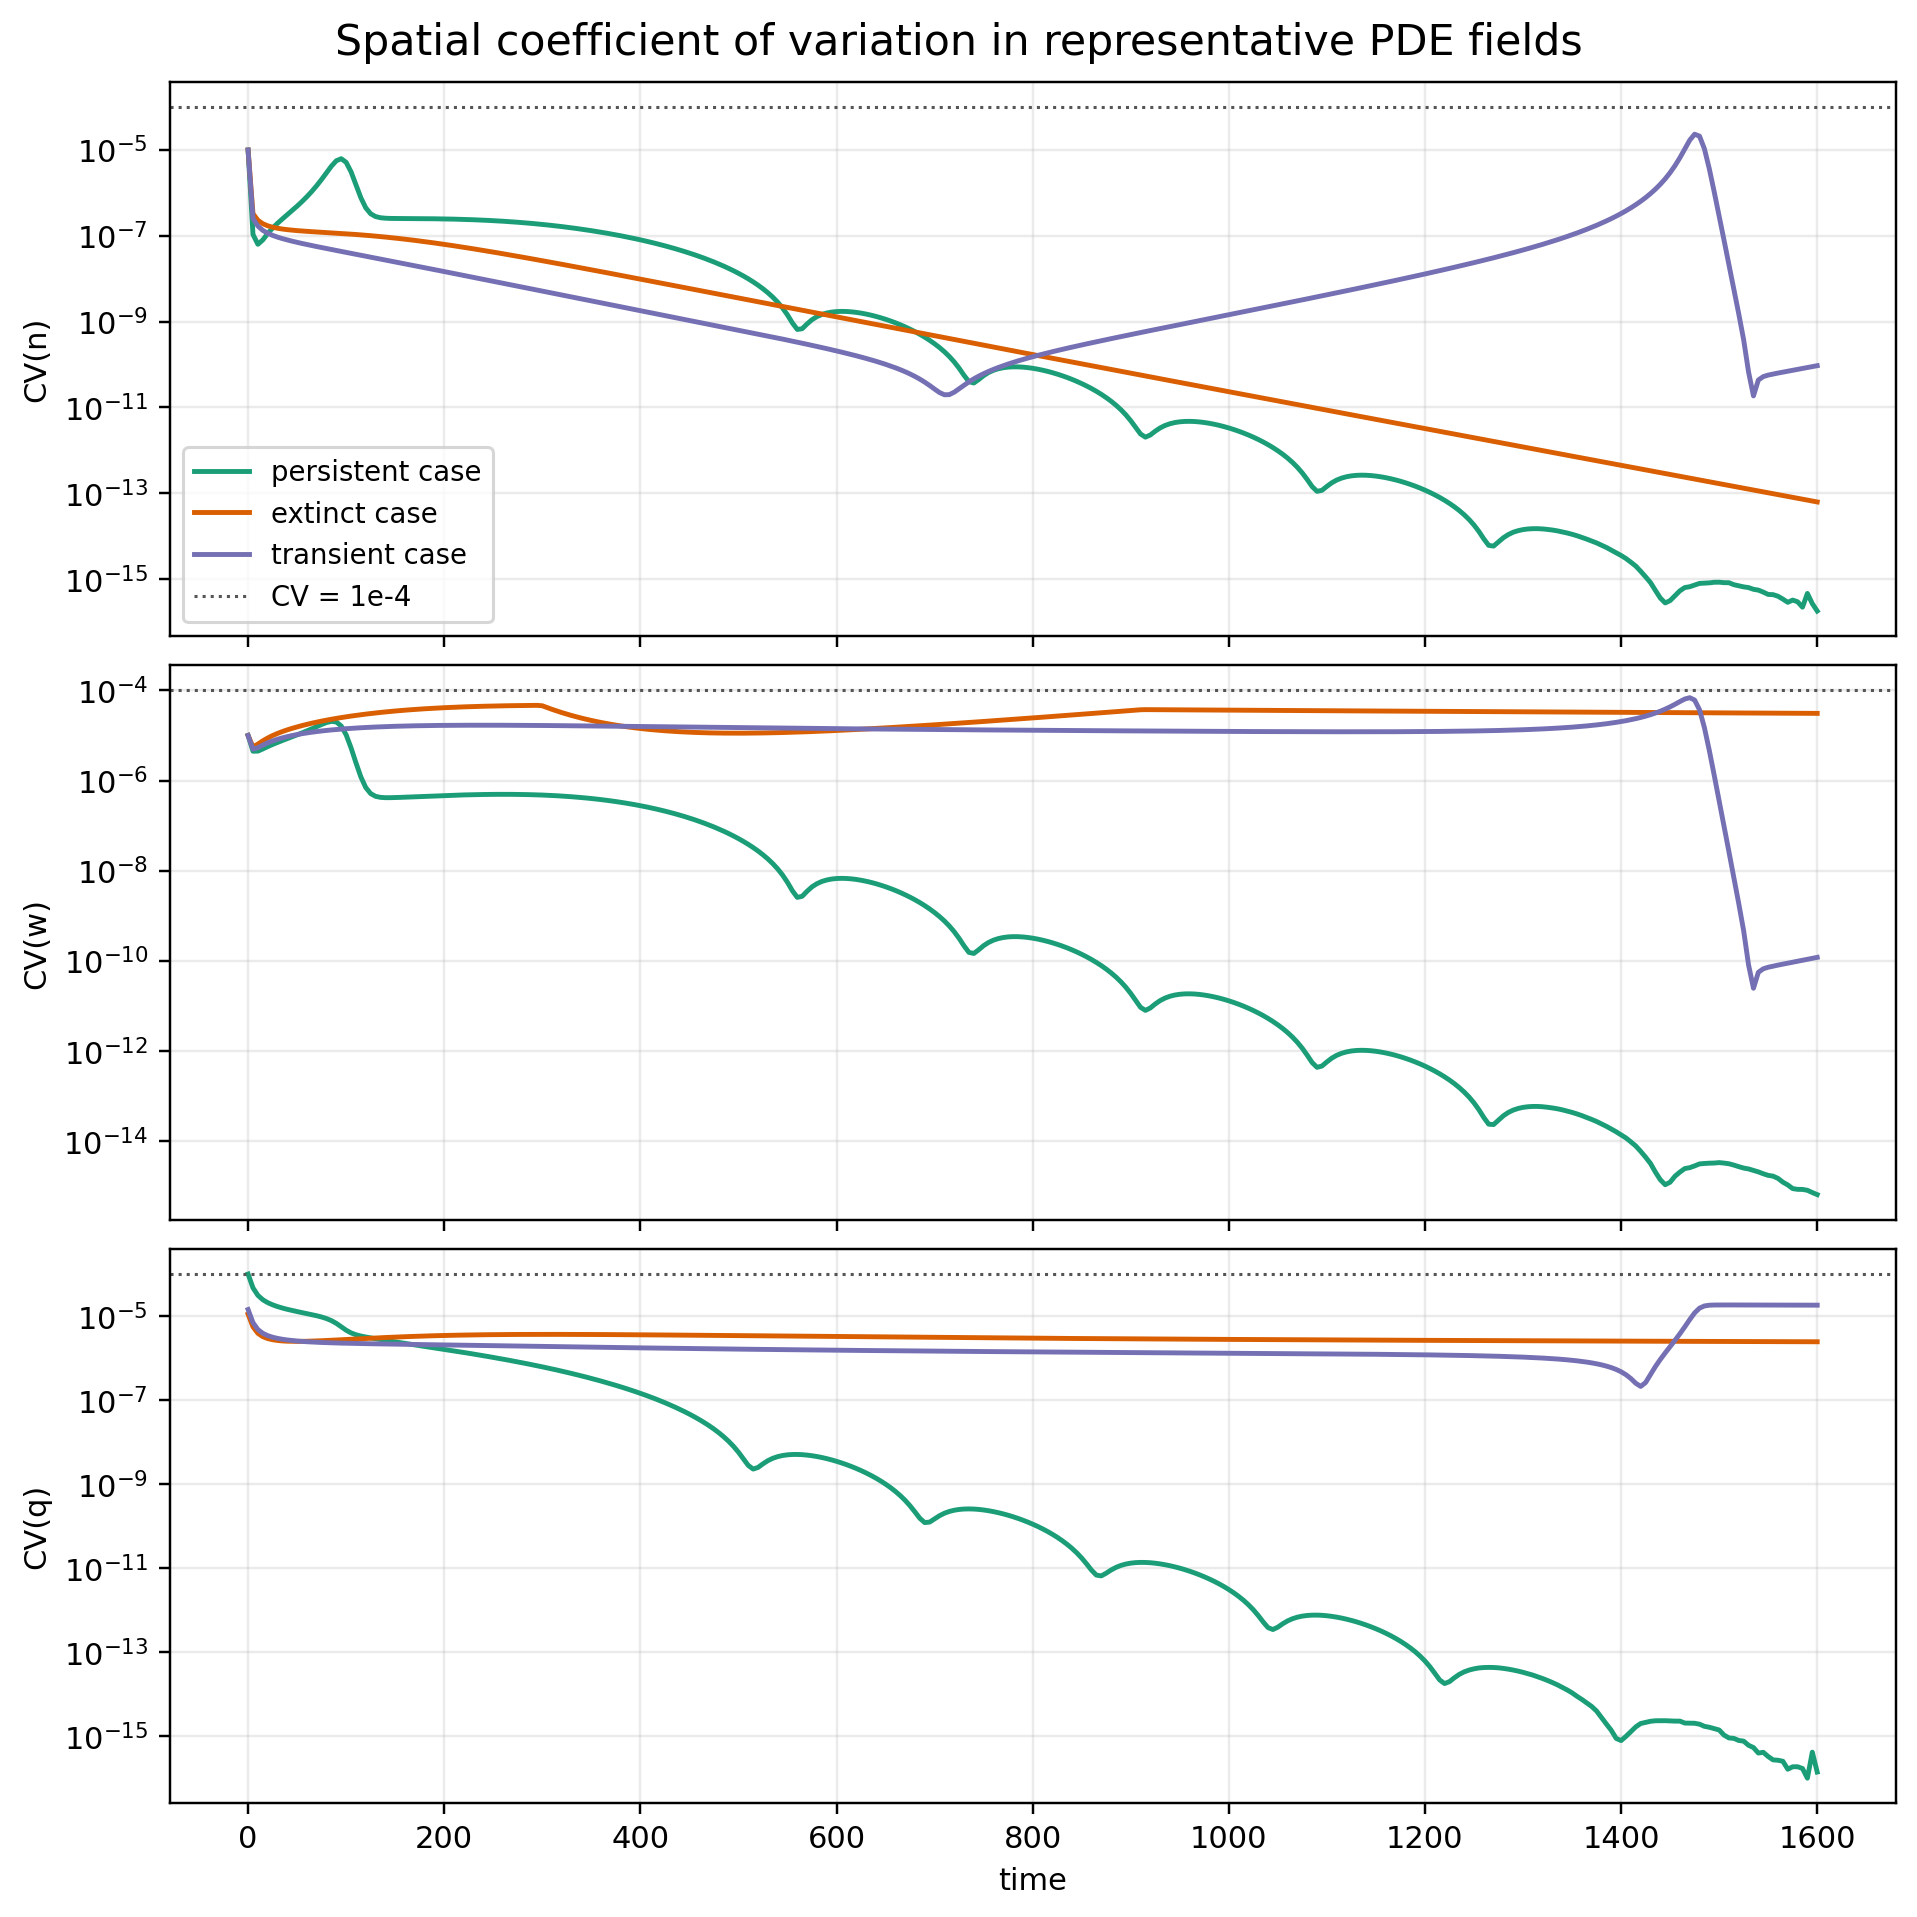
\includegraphics[width=0.82\linewidth]{figures/roy_evo_spatial/report/fig23_spatial_variance_decay.png}
\caption{Spatial coefficient of variation through time for representative PDE cases.}
\end{figure}

\subsection{Basin-label agreement between ODE and PDE}

The ODE/PDE basin-label agreement fraction on the existing \(q_0\)--\(w_0\) grid was 0.9 over 140 compared rows. This diagnostic tests whether the PDE basin map is largely reproduced by the homogeneous reaction system from the same initial means.

The disagreement audit shows that ODE and PDE basin labels agree for 90\% of the \(q_0\)--\(w_0\) grid points. Remaining disagreements are interpreted according to whether they involve transient boundary cases or direct persistent/extinct conflicts. In this audit, 14 disagreements involved transient labels and 0 were direct persistent/extinct conflicts.

\begin{figure}[htbp]
\centering
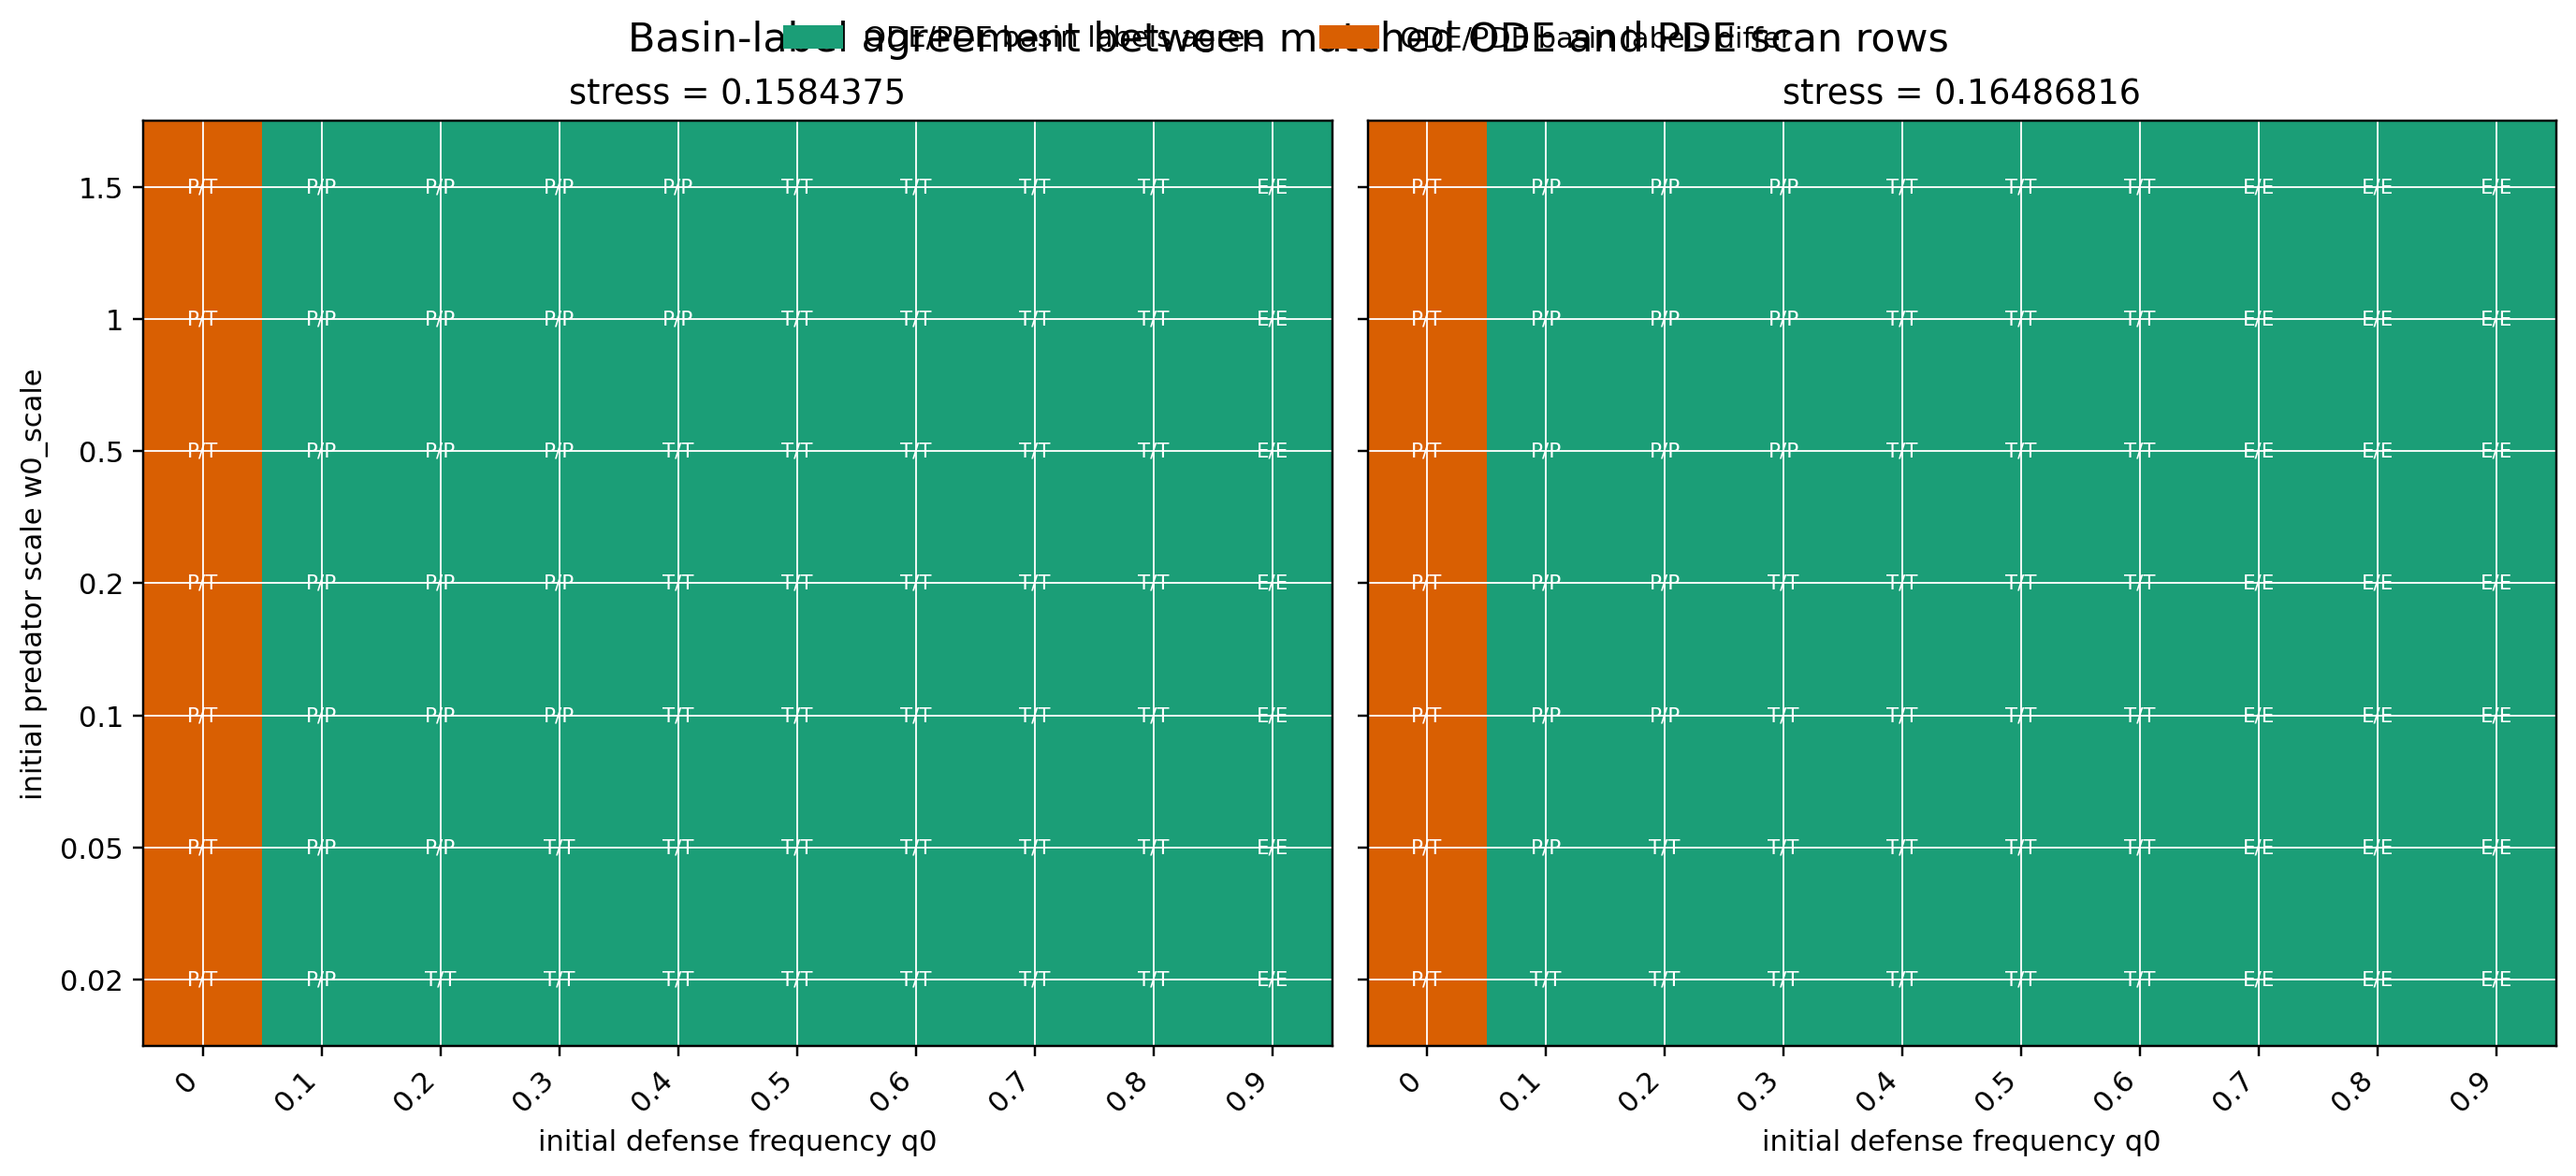
\includegraphics[width=0.98\linewidth]{figures/roy_evo_spatial/report/fig24_ode_pde_basin_agreement.png}
\caption{ODE/PDE basin-label agreement on the existing focused \(q_0\)--\(w_0\) basin grid. Cell labels show ODE/PDE basin initials.}
\end{figure}

\begin{figure}[htbp]
\centering
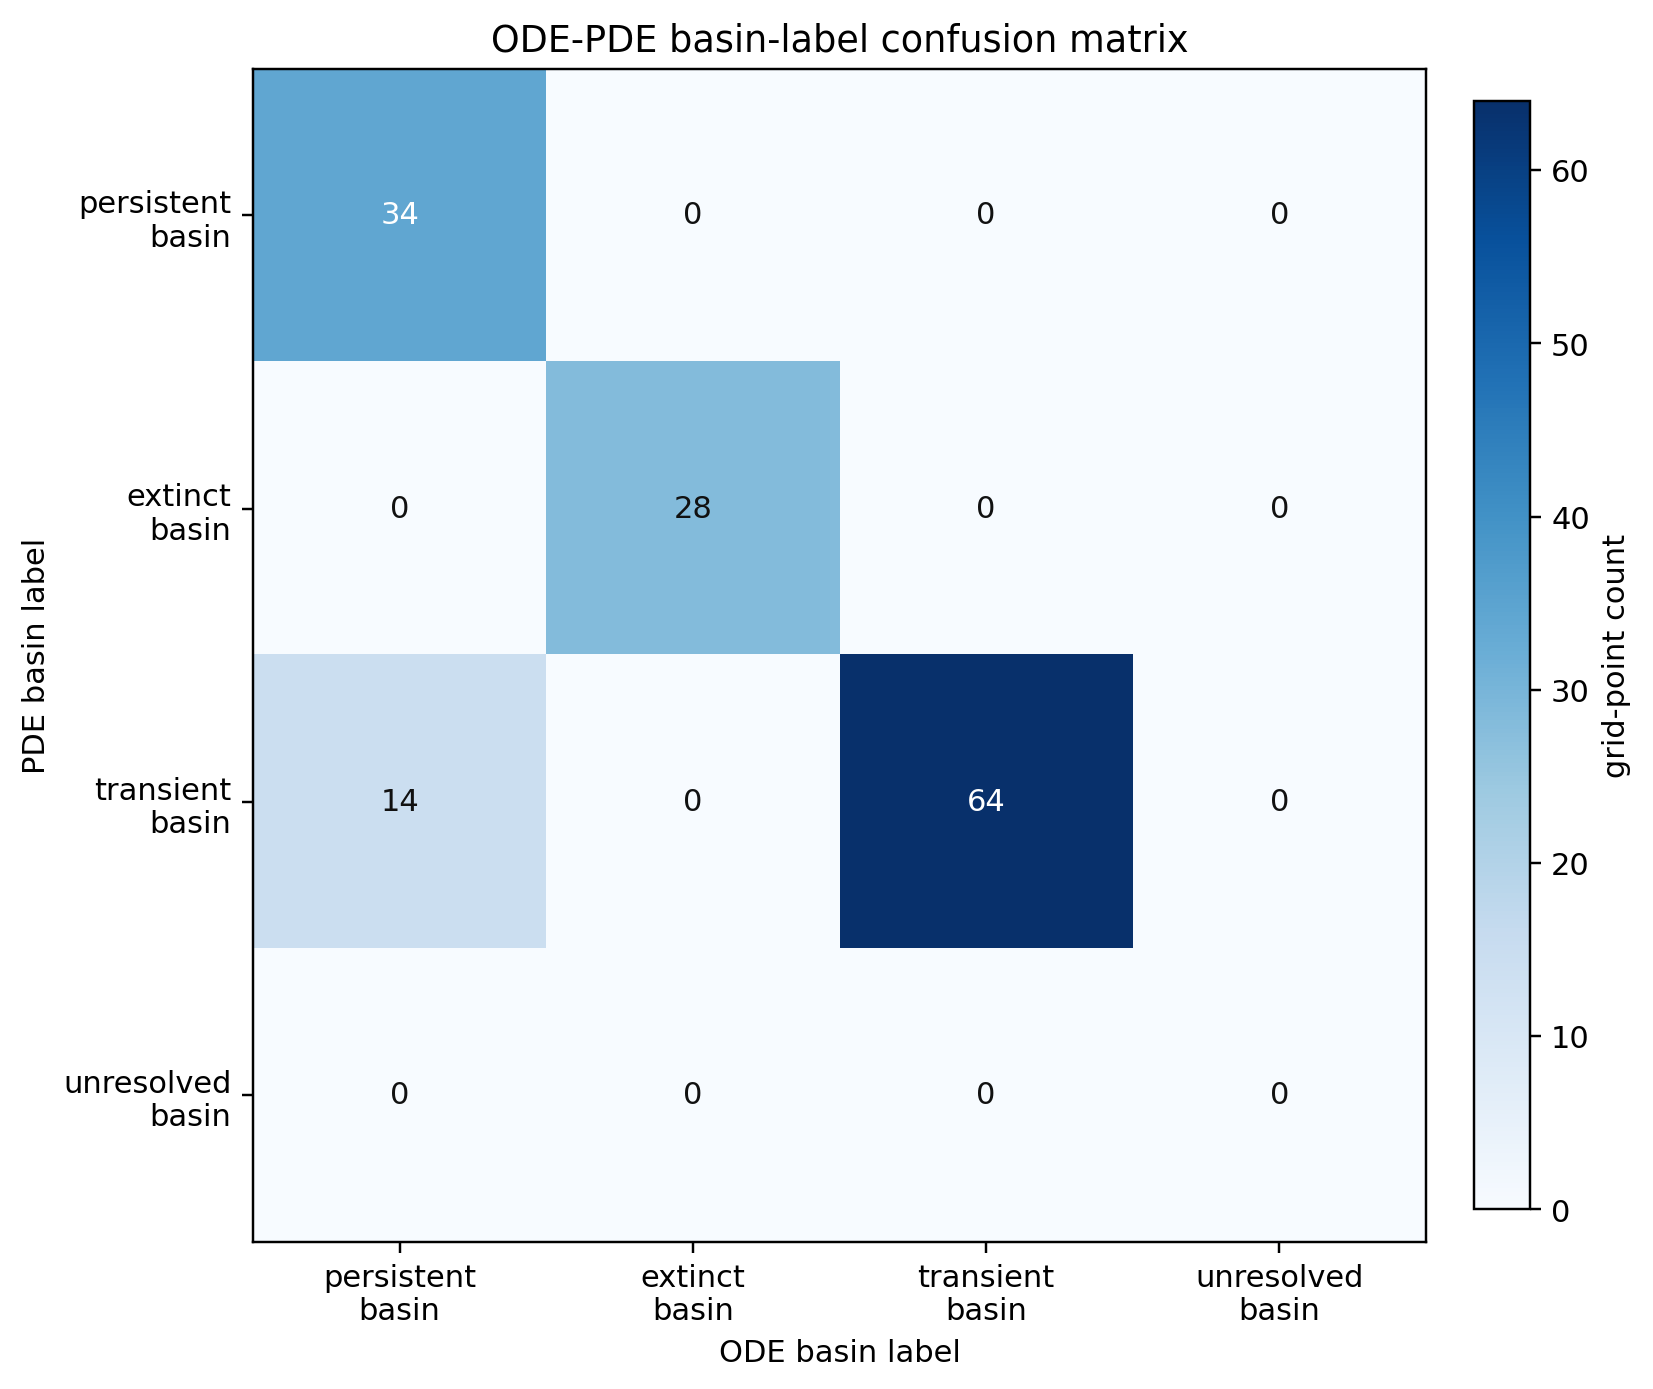
\includegraphics[width=0.72\linewidth]{figures/roy_evo_spatial/report/fig27_ode_pde_basin_confusion_matrix.png}
\caption{Confusion matrix comparing ODE and PDE basin labels across the existing focused \(q_0\)--\(w_0\) grid.}
\end{figure}

\subsection{Perturbation sensitivity}

The perturbation test found 0 outcome-changing case groups out of 3, and 0 outcome-changing groups among the persistent and extinct representative cases.

\begin{figure}[htbp]
\centering
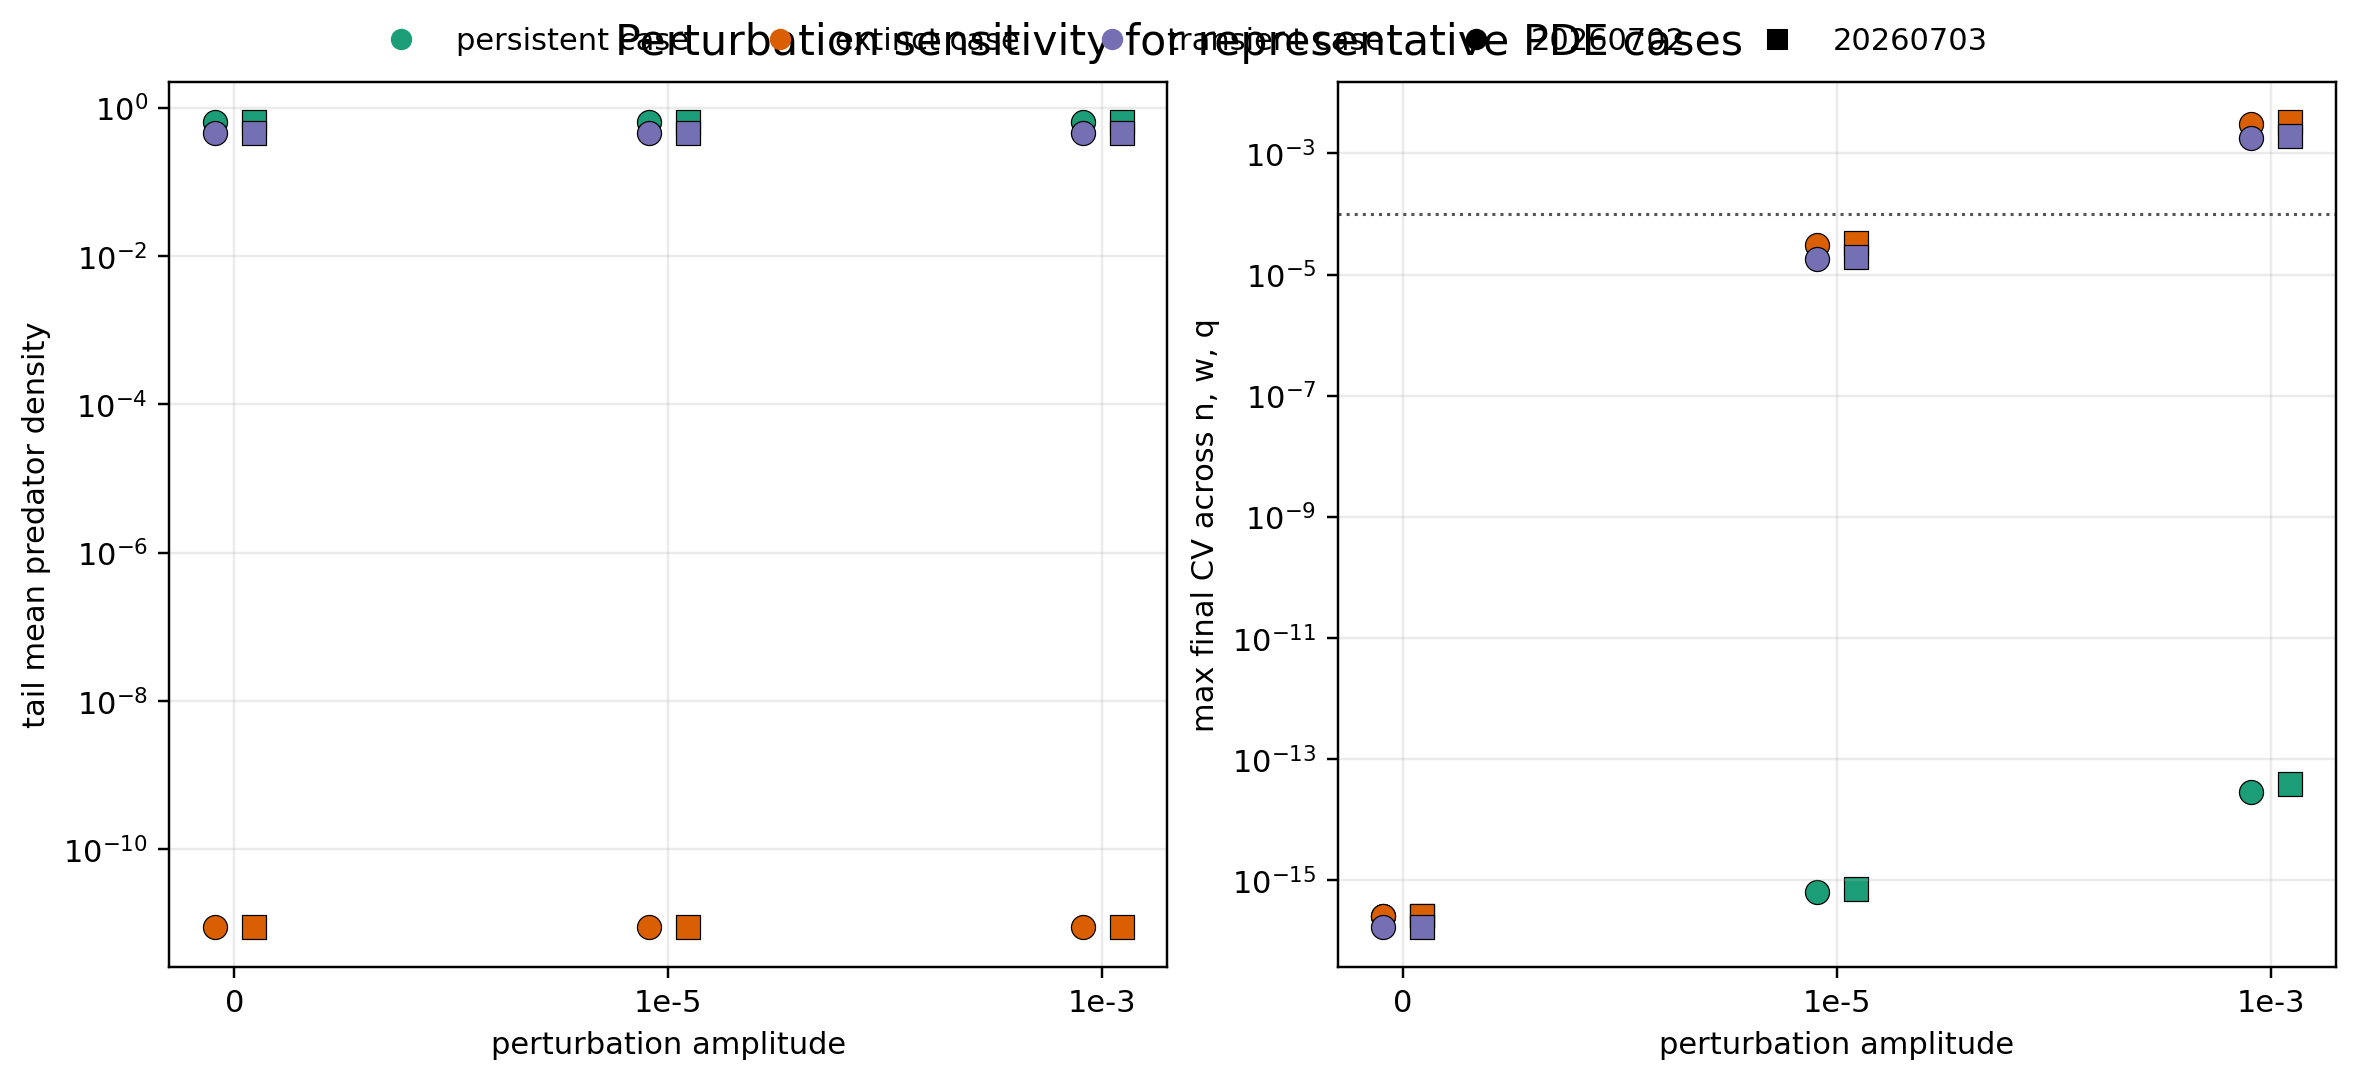
\includegraphics[width=0.90\linewidth]{figures/roy_evo_spatial/report/fig25_perturbation_sensitivity.png}
\caption{Perturbation-amplitude and seed sensitivity for the representative PDE cases.}
\end{figure}

\subsection{Mechanism decision}

The final decision label is
\[
\texttt{reaction\_dominated\_homogeneous\_multistability}.
\]
The current evidence indicates that basin dependence is primarily inherited from homogeneous eco-evolutionary reaction dynamics rather than generated by persistent spatial patterning.

\begin{figure}[htbp]
\centering
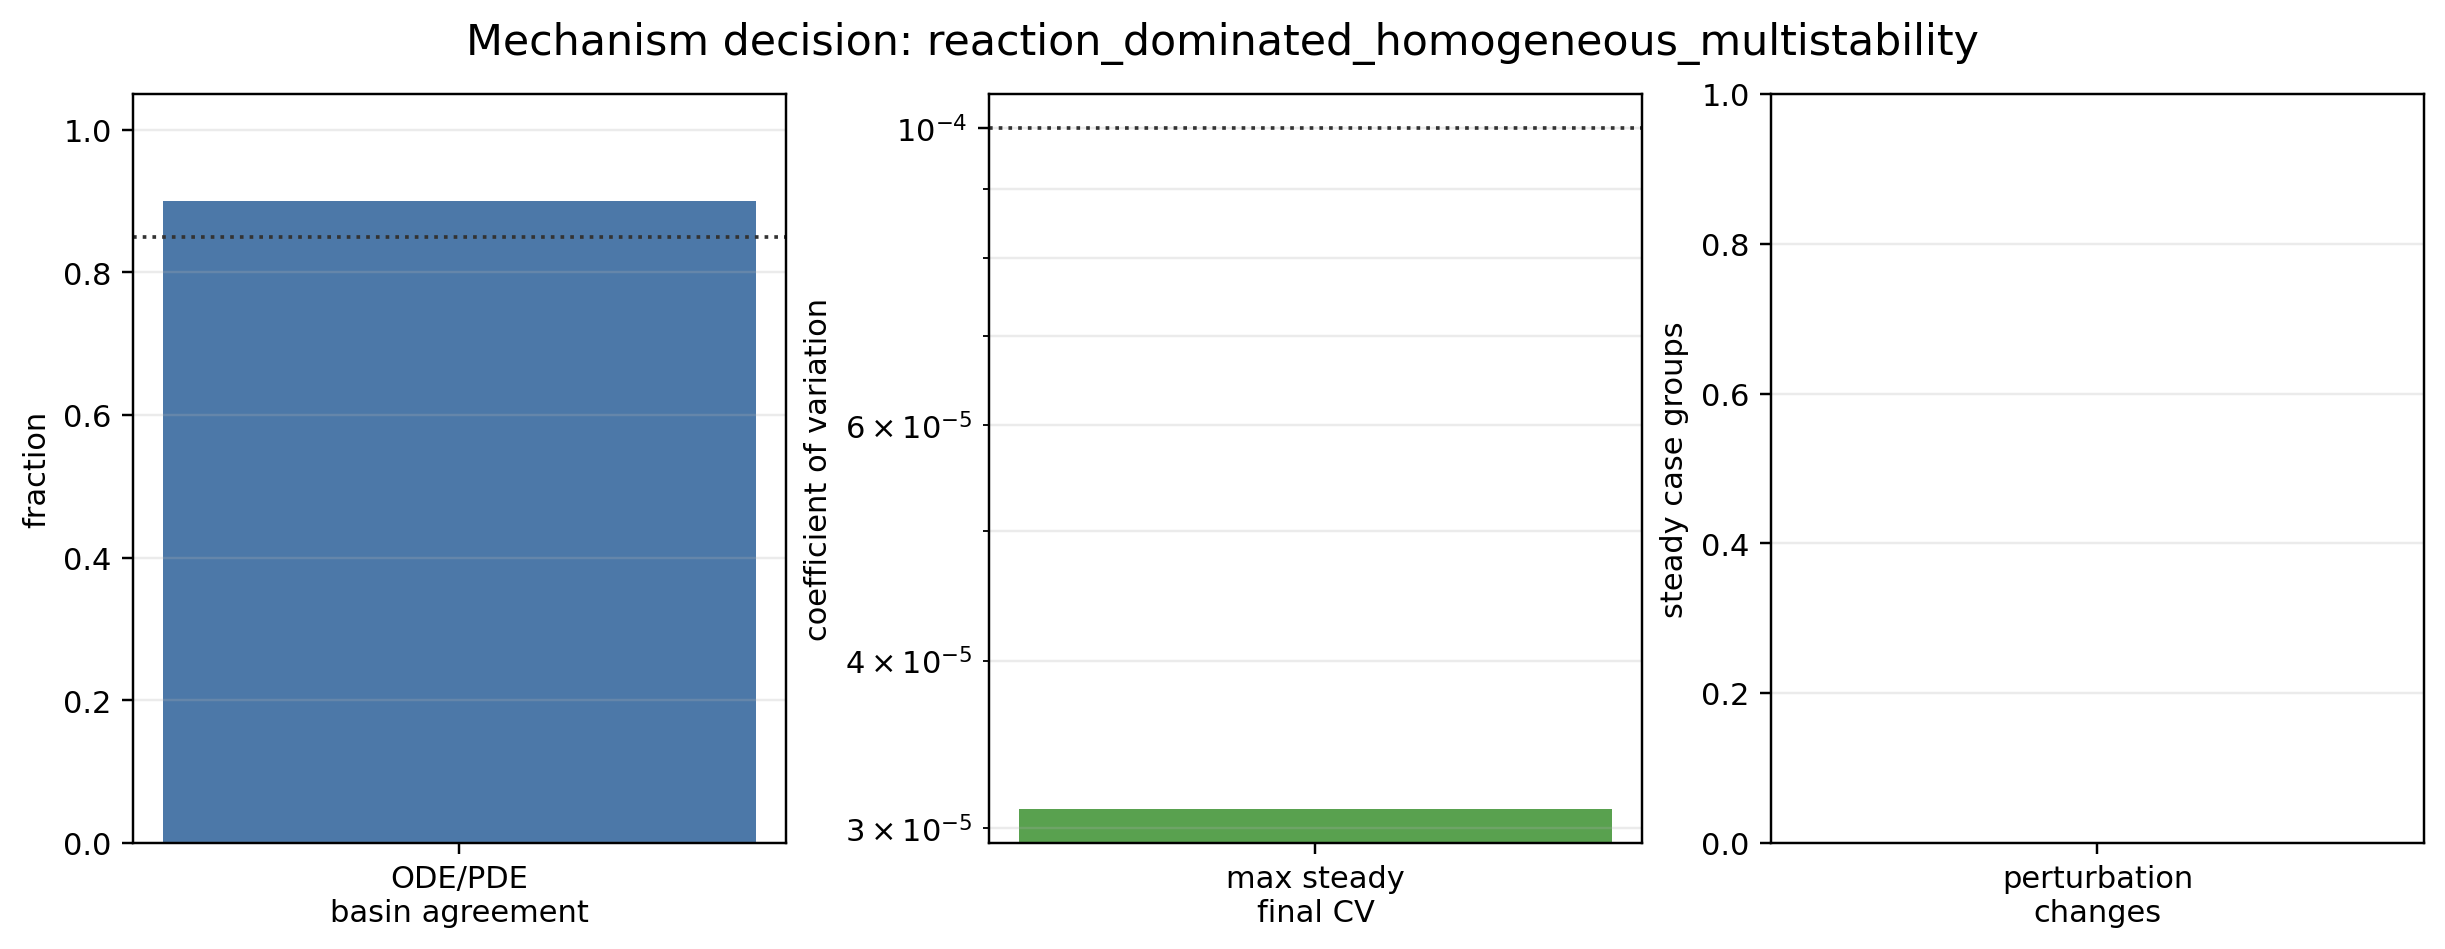
\includegraphics[width=0.92\linewidth]{figures/roy_evo_spatial/report/fig26_mechanism_decision_summary.png}
\caption{Compact summary of the mechanism decision diagnostics.}
\end{figure}

\section{Biological interpretation}

The analysis explicitly answers the mechanism question: The observed PDE basins are primarily homogeneous reaction-dominated in this tested parameterization. This means that the current basin dependence should be interpreted as an initial-condition dependence of the eco-evolutionary reaction dynamics unless future targeted work reveals stronger spatial patterning or perturbation-sensitive basin entry.

The equilibrium scan suggests that the persistent homogeneous branch compensates increased predator mortality by lowering the equilibrium defense frequency \(q^*\), while \(n^*\) and \(w^*\) remain close to the same positive values over the tested stress range. This provides a reaction-level explanation for the rescue mechanism and for why the spatial PDE can inherit basin-dependent outcomes without persistent spatial patterning.

The mechanism diagnosis points to a homogeneous compensation branch. The persistent branch is explained by the ODE equilibrium conditions, where \(q^*(s)\) shifts downward as stress increases and restores predator growth balance. A follow-up local trade-off check supports this branch in the current parameterization and nearby structured trade-off settings, with supporting diagnostics in Figures 33, 34, and 37 of the main report. The robustness claim remains local and parameter-dependent.

A subsequent conditions analysis makes this mechanism more explicit. For the linear trade-off ODE, the interior branch exists when \(c=(r_v-r_u)/(a_v-a_u)>0\), \(r_u-ca_u>0\), the implied \(z^*,w^*,n^*\) are positive, and the predator-balance value \(q^*(s)\) lies in \((0,1)\). In the current parameterization, these feasibility inequalities hold over the tested stresses, the analytic branch matches the numerical persistent equilibria to machine precision, and the analytic Jacobian is locally stable at the tested target stresses. This strengthens the homogeneous mechanism diagnosis while keeping it conditional on the tested linear trade-offs.

The local stability calculation was also reformulated with the Routh--Hurwitz conditions for the cubic characteristic polynomial of the analytic Jacobian. For \(\lambda^3+A_1\lambda^2+A_2\lambda+A_3\), local stability requires \(A_1>0\), \(A_2>0\), \(A_3>0\), and \(A_1A_2>A_3\). These inequalities hold for the current compensation branch at the target stresses and agree with the analytic eigenvalue calculation.

A subsequent PDE spatial-stability analysis treats the homogeneous ODE branch as a homogeneous PDE steady state. Linear perturbations were evaluated with \(J_F(U^*)-\lambda_{mn}D\), and all tested nonzero Neumann modes were stable under the current diffusion coefficients. Targeted finite-amplitude tests used localized predator patches, localized defense patches, sinusoidal modes, random heterogeneity, and basin-boundary heterogeneity. The resulting decision is spatial stability of the homogeneous branch with finite-amplitude basin effects: local-defense perturbations from basin-boundary mean states changed finite-horizon basin assignment from persistent to transient, but final spatial CV values decayed below threshold and no sustained spatial pattern persisted. This refines the mechanism diagnosis toward finite-amplitude basin-entry sensitivity near boundary states rather than persistent spatial-pattern-mediated rescue.

\section{Limitations}

The conclusion is restricted to the tested parameterization. The analysis tests the current diffusion coefficients and a controlled linear diffusion-ratio grid, but it does not establish global results over diffusion coefficients, trade-off forms, evolutionary rates, grid convergence, or longer horizons for all transient basin points. Transient classifications remain lower-confidence than the persistent and extinct steady cases. No general claim is made that spatial structure cannot mediate bistability in other parameter regimes.

\section{Conclusion}

The saved representative PDE fields are close to homogeneous, matched ODE trajectories reproduce the relevant mean dynamics, and the basin-grid and perturbation diagnostics provide the decision basis recorded above. Are the observed PDE basins primarily spatially mediated, or primarily homogeneous reaction-dominated? The observed PDE basins are primarily homogeneous reaction-dominated in this tested parameterization, with an added caveat that finite-amplitude heterogeneity can shift finite-horizon basin labels near tested boundary states without producing persistent spatial patterning.

A follow-up homogeneous ODE mechanism analysis now treats the reaction system as the primary object of study. It computes representative ODE trajectories, selection-gradient and predator-growth diagnostics, an ODE \(q_0\)--\(w_0\) basin map, and numerical equilibria with finite-difference stability labels. Those results support the interpretation that the current PDE basin structure is inherited from homogeneous eco-evolutionary reaction dynamics, while keeping the conclusion conditional on the tested trade-off parameterization.

\end{document}
